\documentclass{article}
\usepackage[utf8]{inputenc}
\usepackage[super,square]{natbib}
\usepackage{tabularx}
\usepackage{parskip}
\usepackage[margin=1.4in]{geometry}
\usepackage{csquotes}
\usepackage{amsmath}
\usepackage{amsfonts}
\usepackage{amsthm}
\usepackage{graphicx}
\usepackage{float}
\usepackage{hyperref}
\usepackage{xcolor,listings}
\usepackage{textcomp}
\usepackage{multicol}

\newcommand{\comment}[1]{}

\lstset{upquote=true}

\definecolor{backcolour}{rgb}{0.95,0.95,0.92}
\definecolor{codegray}{rgb}{0.5,0.5,0.5}
\definecolor{bluehl}{RGB}{85,136,252}
\lstdefinestyle{mystyle}{
    backgroundcolor=\color{backcolour},
    % keywordstyle=\color{magenta},
    keywordstyle=\color{bluehl},
    showspaces=false,
    basicstyle=\ttfamily,
    numbers=left,
    numberstyle=\tiny\color{codegray},
    numbersep=5pt,
    commentstyle=\color{gray}
}
\lstset{style=mystyle}

\title{\vspace{-3cm} SQL Notes}
\author{}
\date{}
\comment{
    TODO: 
    - Convert all code snippets to PostgreSQL 
    - Convert all code snippets to use same example table
}

\begin{document}

\maketitle
\vspace{-1.5cm}
\tableofcontents
\newpage

\section{Pre-requsite Concepts}

\subsection{ACID}
\textbf{Atomicity} -- ensures that all operations within the work unit are completed successfully. Otherwise, the transaction is aborted at the point of failure and all the previous operations are rolled back to their former state.

\textbf{Consistency} -- ensures that the database properly changes states upon a successfully committed transaction.

\textbf{Isolation} -- enables transactions to operate independently of and transparent to each other.

\textbf{Durability} -- ensures that the result or effect of a committed transaction persists in case of a system failure.


\subsection{Types of SQL Commands}
SQL commands are mainly categorized into four categories as:
\begin{enumerate}
    \item DDL -- Data Definition Language
    \item DQl -- Data Query Language
    \item DML -- Data Manipulation Language
    \item DCL -- Data Control Language
    \item TCL -- Transaction Control Language
\end{enumerate}

\begin{figure}[h]
    \centering
    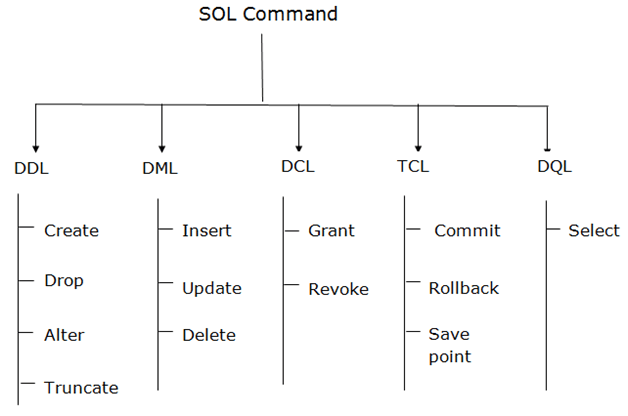
\includegraphics[width=14cm]{dbms-sql-command.png}
\end{figure}


\newpage
\section{Reading Data}
\subsection{SELECT Statement}
\subsubsection{Select all}

\vspace{8pt}
\begin{lstlisting}[language=SQL]
SELECT *
FROM students;
\end{lstlisting} \vspace{8pt}

\subsubsection{Select specific columns}
\vspace{8pt} \begin{lstlisting}[language=SQL]
SELECT name, age
FROM students;
\end{lstlisting} \vspace{8pt}

\subsubsection{De-duplicate rows}

\vspace{8pt} \begin{lstlisting}[language=SQL]
SELECT DISTINCT name
FROM students;
\end{lstlisting} \vspace{8pt}


\subsubsection{Aliasing}

In the SELECT block, $<$expression$>$ AS $<$alias$>$ provides an alias that can be referred to later in the query. This saves us from having to write out long expressions again, and can clarify the purpose of the expression.

\vspace{8pt} \begin{lstlisting}[language=SQL]
SELECT name, age, location AS personal_info
FROM students;
\end{lstlisting}


\subsection{WHERE, Conditions and Comparators}
\subsubsection{Numeric comparison}

\vspace{8pt} \begin{lstlisting}[language=SQL]
=    /* equals */
<    /* less-than */
<=   /* less-than or equals */
>    /* greater-than */
>=   /* greater-than or equals */
!=   /* does not equal */
<>   /* does not equal */
\end{lstlisting} \vspace{8pt}

\subsubsection{String comparison}

Note that string values in the condition should be put between single quotes. Also note that any uppercase letter is smaller (i.e. comes before) any lowercase letter.

\vspace{8pt} \begin{lstlisting}[language=SQL]
=    /* equals */
<    /* before in dictionary order */
<=   /* before or the same */
>    /* after in dictionary order */
>=   /* after or the same */
!=   /* does not equal */
<>   /* does not equal */ 
\end{lstlisting} \vspace{8pt}

\subsubsection{AND and OR}

Complex clauses can be made out of simple ones using Boolean operators like NOT, AND and OR. SQL gives most precedence to NOT and then AND and finally OR. But if you’re too lazy to remember the order of precedence, you can use parenthesis to clarify the order you want.

\vspace{8pt} \begin{lstlisting}[language=SQL]
SELECT product
FROM inventory
WHERE amount < 5
OR name = 'paper'
AND price > 1;
\end{lstlisting} \vspace{8pt}

When using both AND and OR it's important to know that AND has higher precedence.

If we want the OR to be evaluated first, we can use brackets ( ).

\vspace{8pt} \begin{lstlisting}[language=SQL]
SELECT product
FROM inventory
WHERE (amount < 5
OR name = 'paper')
AND price > 1;
\end{lstlisting} \vspace{8pt}

\subsubsection{In a given list of values}

\vspace{8pt} \begin{lstlisting}[language=SQL]
SELECT product
FROM inventory
WHERE amount IN (1, 5, 10);
\end{lstlisting} \vspace{8pt}

\subsubsection{Inclusive ranges}

\vspace{8pt} \begin{lstlisting}[language=SQL]
SELECT product
FROM inventory
WHERE amount BETWEEN 5 AND 9;
\end{lstlisting} \vspace{8pt}

is the equivalent condition to

\vspace{8pt} \begin{lstlisting}[language=SQL]
SELECT product
FROM inventory
WHERE amount >= 5 AND amount <= 9
\end{lstlisting} \vspace{8pt}

\subsubsection{Exists, Any, All}

\vspace{8pt} \begin{lstlisting}[language=SQL]
SELECT column_name(s)
FROM table_name
WHERE EXISTS
(SELECT column_name FROM table_name WHERE condition);
\end{lstlisting} \vspace{8pt}

\vspace{8pt} \begin{lstlisting}[language=SQL]
SELECT column_name(s)
FROM table_name
WHERE column_name operator ANY
(SELECT column_name FROM table_name WHERE condition);
\end{lstlisting} \vspace{8pt}

\vspace{8pt} \begin{lstlisting}[language=SQL]
SELECT column_name(s)
FROM table_name
WHERE column_name operator ALL
(SELECT column_name FROM table_name WHERE condition);
\end{lstlisting} \vspace{8pt}

\subsection{String Pattern Matching}
\subsubsection{Quotes}

In SQL, strings are denoted by single quotes. Backticks can be used to denote column and table names. This is useful when the column or table name is the same as a SQL keyword and when they have a space in them.

\subsubsection{LIKE string operators}

The most powerful string operators is probably LIKE. It allows us to use wildcards such as \% and \_ to match various characters. For instance, first\_name LIKE '\%roy' will return true for rows with first names ‘roy’, ‘Troy’, and ‘Deroy’ but not ‘royman’. The wildcard \_ will match a single character so first\_name LIKE '\_roy' will only match ‘Troy’.

\vspace{8pt} \begin{lstlisting}[language=SQL]
SELECT first_name, last_name, ex_number
FROM executions
WHERE first_name = 'Raymond'
  AND last_name LIKE '%Landry%'
\end{lstlisting} \vspace{8pt}


\subsection{Operations on Retrieved Records}
\subsubsection{Sort rows}

\vspace{8pt} \begin{lstlisting}[language=SQL]
SELECT name, age
FROM friends
ORDER BY name, age DESC, last_name ASC;
\end{lstlisting} \vspace{8pt}

\subsubsection{Limit the number of rows}

\vspace{8pt} \begin{lstlisting}[language=SQL]
SELECT name, grade
FROM course_grades
ORDER BY grade DESC
LIMIT 5;
\end{lstlisting} \vspace{8pt}

\subsubsection{Filter rows}

\vspace{8pt} \begin{lstlisting}[language=SQL]
SELECT product
FROM inventory
WHERE code = 'ABC123';
\end{lstlisting} \vspace{8pt}


\subsection{Aggregate Functions }

To aggregate means to combine multiple elements into a whole. Similarly, aggregation functions take multiple rows of data and combine them into one number.

\subsubsection{The COUNT Function}

COUNT($<$column$>$) returns the number of non-null rows in the column.

\vspace{8pt} \begin{lstlisting}[language=SQL]
SELECT COUNT(first_name) FROM executions
\end{lstlisting} \vspace{8pt}

\subsubsection{NULLS}

In SQL, NULL is the value of an empty entry. This is different from the empty string `' and the integer 0, both of which are not considered NULL. To check if an entry is NULL, use IS and IS NOT instead of = and !=.

What if we don’t know which columns are NULL-free? Worse still, what if none of the columns are NULL-free?  The solution is COUNT(\*). This is reminiscent of SELECT \* where the \* represents all columns. In practice COUNT(\*) counts rows as long as any one of their columns is non-null. This helps us find table lengths because a table shouldn’t have rows that are completely null.

\vspace{8pt} \begin{lstlisting}[language=SQL]
SELECT COUNT(*) FROM executions
\end{lstlisting} \vspace{8pt}

\subsubsection{Subsets}
Another common variation is to count a subset of the table. For instance, counting Harris county executions.

\vspace{8pt} \begin{lstlisting}[language=SQL]
SELECT COUNT(*) FROM executions WHERE county='Harris'
\end{lstlisting} \vspace{8pt}

\subsubsection{Cumulative Sum}

Write a query to get cumulative cash flow for each day such that we end up with a table in the form below: 

\vspace{8pt} \begin{lstlisting}[language=SQL]
/*
| date       | cumulative_cf |
|------------|---------------|
| 2018-01-01 | -1000         |
| 2018-01-03 | -1050         |
| ...        | ...           |
*/
SELECT 
    a.date date, 
    SUM(b.cash_flow) as cumulative_cf 
FROM
    transactions a
JOIN b 
    transactions b ON a.date >= b.date 
GROUP BY 
    a.date 
ORDER BY 
    date ASC
/* 
    Alternate solution using a window function (more efficient!)
*/

SELECT 
    date, 
    SUM(cash_flow) OVER (ORDER BY date ASC) as cumulative_cf 
FROM
    transactions 
ORDER BY 
    date ASC
\end{lstlisting} \vspace{8pt}

\subsubsection{CASE WHEN }

What if we want to simultaneously find the number of Bexar county executions? The solution is to apply a CASE WHEN block which acts as a big if-else statement.

\vspace{8pt} \begin{lstlisting}[language=SQL]
CASE
    WHEN <clause> THEN <result>
    WHEN <clause> THEN <result>
    ...
    ELSE <result>
END
\end{lstlisting} \vspace{8pt}

A common mistake is to miss out the END command and the ELSE condition which is a catchall in case all the prior clauses are false. Also recall that clauses are expressions that can be evaluated to be true or false. This makes it important to think about the boolean value of whatever you stuff in there.

\vspace{8pt} \begin{lstlisting}[language=SQL]
SELECT
    SUM(CASE WHEN county='Harris' THEN 1
        ELSE 0 END),
    SUM(CASE WHEN county='Bexar' THEN 1
        ELSE 0 END)
FROM executions
\end{lstlisting} \vspace{8pt}

\vspace{8pt} \begin{lstlisting}[language=SQL]
SELECT
    COUNT(CASE WHEN county='Harris' THEN 1
        ELSE NULL END),
    COUNT(CASE WHEN county='Bexar' THEN 1
        ELSE NULL END)
FROM executions
\end{lstlisting} \vspace{8pt}

\begin{enumerate}
    \item With a WHERE block,
    \item With a COUNT and CASE WHEN block,
    \item With two COUNT functions.
\end{enumerate}

The WHERE version had it filter down to a small table first before aggregating while in the other two, it had to look through the full table. In the COUNT + CASE WHEN version, it only had to go through once, while the double COUNT version made it go through twice. So even though the output was identical, the performance was probably best in the first and worse in the other versions.

\subsubsection{The GROUP BY Block}

The GROUP BY block allows us to split up the dataset and apply aggregate functions within each group, resulting in one row per group. Its most basic form is GROUP BY $<$column$>$, $<$column$>$, ... and comes after the WHERE block.

\vspace{8pt} \begin{lstlisting}[language=SQL]
SELECT
  county,
  COUNT(*) AS county_executions
FROM executions
GROUP BY county
\end{lstlisting} \vspace{8pt}

Filtering via the WHERE block happens before grouping and aggregation. This is reflected in the order of syntax. After all, the WHERE block always precedes the GROUP BY block.

We generally do not want to mix aggregated and non-aggregated columns. The difference here is that grouping columns are the only columns allowed to be non-aggregate. After all, all the rows in that group must have the same values on those columns so there’s no ambiguity in the value that should be returned.

\subsubsection{The HAVING Block }

What happens if we want to filter on the result of the grouping and aggregation? Surely we can’t jump forward into the future and grab information from there. To solve this problem, we use HAVING.

We need an additional filter—one that uses the result of the aggregation. This means it cannot exist in the WHERE block because those filters are run before aggregation. You can think of it as a post-aggregation WHERE block.

\vspace{8pt} \begin{lstlisting}[language=SQL]
SELECT county
FROM executions
WHERE ex_age >= 50
GROUP BY county
HAVING COUNT(*) > 2
\end{lstlisting} \vspace{8pt}

\subsubsection{Averages}

Note: you can compose functions.

\vspace{8pt} \begin{lstlisting}[language=SQL]
SELECT AVG(LENGTH(last_statement)) FROM executions
\end{lstlisting} \vspace{8pt}


\subsubsection{Rolling Average}
To write a query to get 7-day rolling (preceding) average of daily sign ups.

\vspace{8pt} \begin{lstlisting}[language=SQL]
/*
| date       | sign_ups |
|------------|----------|
| 2018-01-01 | 10       |
| 2018-01-02 | 20       |
| 2018-01-03 | 50       |
| ...        | ...      |
| 2018-10-01 | 35       |
*/

SELECT 
  a.date, 
  AVG(b.sign_ups) average_sign_ups 
FROM 
  signups a 
JOIN 
  signups b 
  ON a.date <= b.date + interval '6 days' 
  AND a.date >= b.date
GROUP BY 
  a.date
\end{lstlisting} \vspace{8pt}

\subsubsection{Percentage}

To calculate percentages, we need two separate queries, one which aggregates with a GROUP BY (to get the numerator) and another that aggregates without (to get the denominator). 

\vspace{8pt} \begin{lstlisting}[language=SQL]
SELECT
  county,
  100.0 * COUNT(*) / (SELECT COUNT(*) FROM executions)
    AS percentage
FROM executions
GROUP BY county
ORDER BY percentage DESC
\end{lstlisting} \vspace{8pt}

\subsubsection{MoM Percent Change}
Find the month-over-month percentage change for monthly active users (MAU).

\vspace{8pt} \begin{lstlisting}[language=SQL]
/*
| user_id | date       |
|---------|------------|
| 1       | 2018-07-01 |
| 3       | 2018-07-02 |
| ...     | ...        |
| 234     | 2018-10-04 |
*/

WITH mau AS 
(
  SELECT 
    DATE_TRUNC('month', date) month_timestamp,
    COUNT(DISTINCT user_id) mau
  FROM 
    logins 
  GROUP BY 
    DATE_TRUNC('month', date)
  )
 SELECT 
    a.month_timestamp previous_month, 
    a.mau previous_mau, 
    b.month_timestamp current_month, 
    b.mau current_mau, 
    ROUND(100.0*(b.mau - a.mau)/a.mau,2) AS percent_change 
 FROM
    mau a 
 JOIN 
    mau b ON a.month_timestamp = b.month_timestamp 
        - interval '1 month' 
\end{lstlisting}

\subsubsection{Retained Users Per Month}

\vspace{8pt} \begin{lstlisting}[language=SQL]
SELECT 
    DATE_TRUNC('month', a.date) month_timestamp, 
    COUNT(DISTINCT a.user_id) retained_users 
 FROM 
    logins a 
 JOIN 
    logins b ON a.user_id = b.user_id 
        AND DATE_TRUNC('month', a.date) = 
        DATE_TRUNC('month', b.date)  + interval '1 month'
 GROUP BY 
    date_trunc('month', a.date)
\end{lstlisting}

\subsection{Joining Tables}
\subsubsection{Nested Queries}
We can combine multiple queries using a technique called ``nesting”. The parentheses are important for demarcating the boundary between the inner query and the outer one:

\vspace{8pt} \begin{lstlisting}[language=SQL]
SELECT first_name, last_name
FROM executions
WHERE LENGTH(last_statement) =
    (SELECT MAX(LENGTH(last_statement))
     FROM executions)
\end{lstlisting} \vspace{8pt}

\subsubsection{MapReduce}

An interesting addendum is that we've actually just learned to do MapReduce in SQL, i.e. how to map various operations out to all the rows. For example, SELECT LENGTH(last\_statement) FROM executions maps the length function out to all the rows.

\subsubsection{Union}

The UNION operator is used to combine the result-set of two or more SELECT statements. Each SELECT statement within UNION must have the same number of columns. The columns must also have similar data types. The columns in each SELECT statement must also be in the same order. The UNION operator selects only distinct values by default. 

To allow duplicate values, use UNION ALL.

\vspace{8pt} \begin{lstlisting}[language=SQL]
SELECT column_name(s) FROM table_name1
UNION
SELECT column_name(s) FROM table_name2

SELECT column_name(s) FROM table_name1
UNION ALL
SELECT column_name(s) FROM table_name2
\end{lstlisting} \vspace{8pt}

\subsubsection{Joins}

If we wish to combine data from multiple queries but our desired table has the same length as the original executions table, we can rule out aggregations which produce a smaller table.

JOIN creates a big combined table which is then fed into the FROM block just like any other table. The big idea behind JOINs is to create an augmented table because the original doesn't contain the information we need. 

This is a powerful concept because it frees us from the limitations of a single table and allows us to combine multiple tables in potentially complex ways. We’ve also seen that with this extra complexity, meticulous bookkeeping becomes important. Aliasing tables, renaming columns and defining good JOIN ON clauses are all techniques that help us maintain order.

\vspace{8pt} \begin{lstlisting}[language=SQL]
SELECT
  last_ex_date AS start,
  ex_date AS end,
  ex_date - last_ex_date AS day_difference
FROM executions
JOIN previous
  ON executions.ex_number = previous.ex_number
ORDER BY day_difference DESC
LIMIT 10
\end{lstlisting} \vspace{8pt}

\vspace{8pt} \begin{lstlisting}[language=SQL]
SELECT
  last_ex_date AS start,
  ex_date AS end,
  JULIANDAY(ex_date) - JULIANDAY(last_ex_date)
    AS day_difference
FROM executions
JOIN previous
  ON executions.ex_number = previous.ex_number
ORDER BY day_difference DESC
LIMIT 5
\end{lstlisting} \vspace{8pt}

The query above is also notable because the clause executions.ex\_number = previous.ex\_number uses the format $<$table$>$.$<$column$>$ to specify columns. This is only necessary here because both tables have a column called ex\_number.

The JOIN block takes the form of $<$table1$>$ JOIN $<$table2$>$ ON $<$clause$>$. The clause works the same way as in WHERE $<$clause$>$. That is, it is a statement that evaluates to true or false, and anytime a row from the first table and another from the second line up with the clause being true, the two are matched.

The JOIN command defaults to performing what is called an ``inner join” in which unmatched rows are dropped.

To preserve all the rows of the left table, we use a LEFT JOIN in in place of the vanilla JOIN. The empty parts of the row are left alone, which means they evaluate to NULL.

The RIGHT JOIN can be used to preserve unmatched rows in the right table, and the OUTER JOIN can be used to preserve unmatched rows in both.

The final subtlety is handling multiple matches. The join creates enough rows of executions so that each matching row of duplicated\_previous gets its own partner. In this way, joins can create tables that are larger than the their constituents.

\subsubsection{Self Joins }

Remember to use aliases to form the column names (ex\_number, last\_ex\_date). Notice that we are using a table alias here, naming the result of the nested query ``previous".

\vspace{8pt} \begin{lstlisting}[language=SQL]
SELECT
  last_ex_date AS start,
  ex_date AS end,
  JULIANDAY(ex_date) - JULIANDAY(last_ex_date) AS day_difference
FROM executions
JOIN (
    SELECT
      ex_number + 1 AS ex_number,
      ex_date AS last_ex_date
    FROM executions
  ) previous
  ON executions.ex_number = previous.ex_number
ORDER BY day_difference DESC
LIMIT 10
\end{lstlisting} \vspace{8pt}

``previous'' is derived from executions, so we’re effectively joining executions to itself. This is called a ``self join” and is a powerful technique for allowing rows to get information from other parts of the same table.

We've created the previous table to clarify the purpose that it serves. But we can actually write the query more elegantly by joining the executions table directly to itself. Note that we still need to give one copy an alias to ensure that we can refer to it unambiguously.

\vspace{8pt} \begin{lstlisting}[language=SQL]
SELECT
  previous.ex_date AS start,
  executions.ex_date AS end,
  JULIANDAY(executions.ex_date) - JULIANDAY(previous.ex_date)
    AS day_difference
FROM executions
JOIN executions previous
  ON executions.ex_number = previous.ex_number + 1
ORDER BY day_difference DESC
LIMIT 10
\end{lstlisting} \vspace{8pt}

\subsubsection{Multiple Join Conditions}

Write a query to get the response time per email (id) sent to zach@g.com. Do not include ids that did not receive a response from zach@g.com. Assume each email thread has a unique subject. Keep in mind a thread may have multiple responses back-and-forth between zach@g.com and another email address. 

\vspace{8pt} \begin{lstlisting}[language=SQL]
/*
| id | subject  | from         | to           | timestamp      |
|----|----------|--------------|--------------|----------------|
| 1  | Yosemite | zach@g.com   | thomas@g.com | 01-02 12:45:03 |
| 2  | Yosemite | thomas@g.com | zach@g.com   | 01-02 16:35:04 |
| .. | ..       | ..           | ..           | ..             |
*/
SELECT 
    a.id, 
    MIN(b.timestamp) - a.timestamp as time_to_respond 
FROM 
    emails a 
JOIN
    emails b 
        ON 
            b.subject = a.subject 
        AND 
            a.to = b.from
        AND 
            a.from = b.to 
        AND 
            a.timestamp < b.timestamp 
 WHERE 
    a.to = 'zach@g.com' 
 GROUP BY 
    a.id 
\end{lstlisting}

\subsubsection{Cross-Joins}
The CROSS JOIN is used to combine each row of the first table with each row of the second table. It is also known as the Cartesian join since it returns the Cartesian product of the sets of rows from the joined tables.

Say we have a table state\_streams where each row is a state and the total number of hours of streaming from a video hosting service. We want to write a query to get the pairs of states with total streaming amounts within 1000 of each other. 

\vspace{8pt} \begin{lstlisting}[language=SQL]
SELECT
    a.state as state_a, 
    b.state as state_b 
 FROM   
    state_streams a
 CROSS JOIN 
    state_streams b 
 WHERE 
    ABS(a.total_streams - b.total_streams) < 1000
    AND 
    a.state <> b.state 
\end{lstlisting}


\subsection{Window Function}
A window function performs a calculation across a set of table rows that are somehow related to the current row. This is comparable to the type of calculation that can be done with an aggregate function. But unlike regular aggregate functions, use of a window function does not cause rows to become grouped into a single output row — the rows retain their separate identities.

\subsubsection{Get the ID with the highest value}

Write a query to get the empno with the highest salary. Make sure your solution can handle ties!

\vspace{8pt} \begin{lstlisting}[language=SQL]
/*
  depname  | empno | salary |     
-----------+-------+--------+
 develop   |    11 |   5200 | 
 ...
*/
WITH max_salary AS (
    SELECT 
        MAX(salary) max_salary
    FROM 
        salaries
    )
SELECT 
    s.empno
FROM 
    salaries s
JOIN 
    max_salary ms ON s.salary = ms.max_salary 
    
\end{lstlisting}

\subsection{Materialized Views}
In a materialized view, data is being persisted into a virtual table which is maintained by the SQL Server. Views can be used to encapsulate and index commonly used queries or precompute aggregations in order to improve read performance. 

The database engine recreates the data, using the view's SQL statement, every time a user queries a view. Though this can negatively impact write performance because with each operation, the engine will have to update all of the relevant views.

\vspace{8pt} \begin{lstlisting}[language=SQL]
CREATE VIEW view_name AS
SELECT column1, column2, ...
FROM table_name
WHERE condition;
\end{lstlisting}

\newpage
\section{Writing Data}

\subsection{Databases}
\subsubsection{Create database}

\vspace{8pt} \begin{lstlisting}[language=SQL]
CREATE DATABASE database_name
\end{lstlisting} \vspace{8pt}

\subsubsection{Delete database}
\vspace{8pt} \begin{lstlisting}[language=SQL]
DROP DATABASE database_name
\end{lstlisting} \vspace{8pt}

\subsection{Tables}
\subsubsection{Data types}

Some common data types for columns of a table:
\begin{multicols}{2}
\begin{itemize}
    \item CHAR(size)
    \item VARCHAR(size)
    \item BINARY(size)
    \item TEXT(size)
    \item BLOB(size)
    \item ENUM(val1, val2, val3, ...)
    \item SET(val1, val2, val3, ...)
    \item BIT(size)
    \item BOOL or BOOLEAN
    \item INT(size) or INTEGER(size)
    \item FLOAT(size, d)
    \item DATE
    \item DATETIME(fsp)
    \item TIMESTAMP(fsp)
    \item YEAR
\end{itemize}
\end{multicols}

\subsubsection{Constraints}

SQL constraints are used to specify rules for data in a table and can be specified either when the table is created with the CREATE TABLE statement, or after the table is created with the ALTER TABLE statement.

\begin{itemize}
    \item NOT NULL -- Ensures that a column cannot have a NULL value
    \item UNIQUE -- Ensures that all values in a column are different
    \item PRIMARY KEY -- A combination of a NOT NULL and UNIQUE. Uniquely identifies each row in a table
    \item FOREIGN KEY -- Uniquely identifies a row/record in another table
    \item CHECK -- Ensures that all values in a column satisfies a specific condition
    \item DEFAULT -- Sets a default value for a column when no value is specified
    \item INDEX -- Used to create and retrieve data from the database very quickly
\end{itemize}

\subsubsection{Creating tables}
Each column in a database table is required to have a name and a data type.

\vspace{8pt} \begin{lstlisting}[language=SQL]
CREATE TABLE pet (name VARCHAR(20), owner VARCHAR(20),
       species VARCHAR(20), sex CHAR(1), birth DATE, death DATE)
\end{lstlisting} \vspace{8pt}

\subsubsection{Alter table}

\vspace{8pt} \begin{lstlisting}[language=SQL]
ALTER TABLE table_name
ADD column_name datatype

/* or */

ALTER TABLE table_name
DROP COLUMN column_name
\end{lstlisting} \vspace{8pt}

\subsubsection{Deleting tables}

\vspace{8pt} \begin{lstlisting}[language=SQL]
DELETE FROM table_name
WHERE some_column=some_value

/* Delete full table */
DELETE FROM table_name
DELETE * FROM table_name
\end{lstlisting} \vspace{8pt}



\vspace{8pt} \begin{lstlisting}[language=SQL]
CREATE TABLE table_name (
    column1 datatype constraint,
    column2 datatype constraint,
    column3 datatype constraint,
    ....
);
\end{lstlisting} \vspace{8pt}


\subsection{Indexes}
Indexes are used to retrieve data from the database more quickly than otherwise. The users cannot see the indexes, they are just used to speed up searches/queries

Updating a table with indexes takes more time than updating a table without (because the indexes also need an update). So, only create indexes on columns that will be frequently searched against.

Some recommendations involving indexes are:
\begin{itemize}
    \item disable constraints and indexes during bulk loads.
    \item avoid indexes on columns with low selectivity.
    \item use partial indexes.
    \item index columns with high correlation using BRIN (Block Range Index)
\end{itemize}

\subsubsection{B-Trees}
A B-tree is a self-balancing tree data structure that maintains sorted data and allows searches, sequential access, insertions, and deletions in logarithmic time. B-trees and B+trees are commonly used to create indexes in relational databases.

See Data Structures and Algorithms Notebook \footnote{https://github.com/lukepereira/notebooks} for more details. 

\subsubsection{Create index}
By default, duplicate values are allowed. Use UNIQUE keyword if duplicate values are not allowed.

\vspace{8pt} \begin{lstlisting}[language=SQL]
CREATE INDEX index_name
ON table_name (column1, column2, ...);

CREATE UNIQUE INDEX index_name
ON table_name (column1, column2, ...);
\end{lstlisting} \vspace{8pt}

\subsubsection{Delete index}

\vspace{8pt} \begin{lstlisting}[language=SQL]
/* SQL Server */
DROP INDEX table_name.index_name;

/* MySQL */
ALTER TABLE table_name
DROP INDEX index_name;
\end{lstlisting} \vspace{8pt}

\subsection{Records}

\subsubsection{Insert Records}
It is possible to write the INSERT INTO statement in two ways.

The first way specifies both the column names and the values to be inserted. If you are adding values for all the columns of the table, you do not need to specify the column names in the SQL query.

\vspace{8pt} \begin{lstlisting}[language=SQL]
INSERT INTO table_name (column1, column2, column3, ...)
VALUES (value1, value2, value3, ...);

INSERT INTO table_name
VALUES (value1, value2, value3, ...);
\end{lstlisting} \vspace{8pt}

The next time you load data into a table, think about how the data is going to be queried, and make sure you sort it in a way that indexes used for range scan can benefit from.

\subsubsection{Update Records}
UPDATE is a relatively expensive operation. To speed up an UPDATE command it's best to make sure you only update what needs updating.

\vspace{8pt} \begin{lstlisting}[language=SQL]
/* Likely slower */
UPDATE users SET email = lower(email); 

/* Likely faster */
UPDATE users SET email = lower(email)
WHERE email != lower(email);
\end{lstlisting} \vspace{8pt}

\subsubsection{Delete Records}

\vspace{8pt} \begin{lstlisting}[language=SQL]
DELETE FROM table_name WHERE condition;
\end{lstlisting} \vspace{8pt}

\subsubsection{Copy with select and insert}
Copy all columns into an existing table.

\vspace{8pt} \begin{lstlisting}[language=SQL]
INSERT INTO table2
SELECT * FROM table1
WHERE condition;
\end{lstlisting} \vspace{8pt}

The SELECT INTO statement copies data from one table into a new table.
\vspace{8pt} \begin{lstlisting}[language=SQL]
SELECT *
INTO newtable [IN externaldb]
FROM oldtable
WHERE condition;
\end{lstlisting} \vspace{8pt}

\newpage
\section{Transactions}

Transactional control commands are only used with the DML Commands such as INSERT, UPDATE and DELETE. They cannot be used while creating tables or dropping them because these operations are automatically committed in the database.

\begin{itemize}
    \item COMMIT -- to save the changes.
    \item ROLLBACK -- to roll back the changes.
    \item SAVEPOINT -- creates points within the groups of transactions in which to ROLLBACK.
    \item  SET TRANSACTION -- Places a name on a transaction.
\end{itemize}

\subsection{COMMIT}

The COMMIT command is the transactional command used to save changes invoked by a transaction to the database.

\vspace{8pt} \begin{lstlisting}[language=SQL]
DELETE FROM CUSTOMERS
   WHERE AGE = 25;
COMMIT;
\end{lstlisting} \vspace{8pt}

\subsection{ROLLBACK}

The ROLLBACK command is the transactional command used to undo transactions that have not already been saved to the database. This command can only be used to undo transactions since the last COMMIT or ROLLBACK command was issued.

\vspace{8pt} \begin{lstlisting}[language=SQL]
DELETE FROM CUSTOMERS
   WHERE AGE = 25;
ROLLBACK;
\end{lstlisting} \vspace{8pt}

\subsection{SAVEPOINT}

A SAVEPOINT is a point in a transaction when you can roll the transaction back to a certain point without rolling back the entire transaction.

\vspace{8pt} \begin{lstlisting}[language=SQL]
SAVEPOINT SP1;
/* Savepoint created. */
DELETE FROM CUSTOMERS WHERE ID=1;
/* 1 row deleted. */
SAVEPOINT SP2;
/* Savepoint created. */
DELETE FROM CUSTOMERS WHERE ID=2;
/* 1 row deleted. */
ROLLBACK TO SP2;
\end{lstlisting} \vspace{8pt}

The RELEASE SAVEPOINT command is used to remove a SAVEPOINT that you have created.

\vspace{8pt} \begin{lstlisting}[language=SQL]
RELEASE SAVEPOINT SAVEPOINT_NAME;
\end{lstlisting} \vspace{8pt}


\subsection{SET TRANSACTION}

The SET TRANSACTION command can be used to initiate a database transaction. This command is used to specify characteristics for the transaction that follows. For example, you can specify a transaction to be read only or read write.

\vspace{8pt} \begin{lstlisting}[language=SQL]
SET TRANSACTION [ READ WRITE | READ ONLY ];
\end{lstlisting} \vspace{8pt}




\begin{thebibliography}{}

\bibitem[]{}
https://selectstarsql.com/

\bibitem[]{}
https://www.w3schools.com/sql

\bibitem[]{}
https://www.tutorialspoint.com/sql/sql-transactions.htm

\bibitem[]{}
https://quip.com/2gwZArKuWk7W

\bibitem[]{}
https://hakibenita.com/sql-tricks-application-dba

\bibitem[]{}
https://use-the-index-luke.com/

http://docshare01.docshare.tips/files/29375/293750304.pdf

\end{thebibliography}


\end{document}
